\documentclass[11pt, oneside, numbers=noenddot]{scrbook}

\usepackage{style}

\def\Title{OSI 7 Schichtenmodell}	
\def\Subtitle{Layer 1}


\begin{document}


\titlehead{%
\begin{minipage}[c]{0.20\linewidth}

\includegraphics[width=0.8\linewidth]{htl_c_cmyk_rein.pdf}
\end{minipage}
\begin{minipage}[c]{0.5\linewidth}
\begin{center}
{\bfseries\sffamily\large Höhere  technische  Bundeslehranstalt\\
und  Bundesfachschule\\
{\normalsize im Hermann Fuchs Bundesschulzentrum} }
\end{center}
\end{minipage}
\begin{minipage}[c]{0.2\linewidth}
\hfill 
\includegraphics[width=0.8\linewidth]{htl-bildung-mit-zukunft.png}
\end{minipage}\\
}
\title{\vspace{4em}\Title}

\subtitle{\Subtitle}


\author{\\[2,5em] 
\emph{Erstellt von:} \\[0,5em]
Michel Rögl-Brunner, BEd
}
\date{\vspace{3\baselineskip}\small Letzte Änderung: \todayshort}

\begin{titlepage}	
\maketitle
\end{titlepage}
\IfFileExists{revisions.tex}{\clearpage\input{revisions.tex}}{}
\cleardoublepage
\pdfbookmark[1]{Inhaltsverzeichnis}{toc}
\tableofcontents
\clearpage
\pagenumbering{arabic}

\chapter{OSI-Modell und Layer 1}
\section{Grundlagen des OSI-Modells}
Das OSI-Modell (\textit{Open Systems Interconnection Model}) ist ein Referenzmodell, das die Netzwerkkommunikation in sieben klar getrennte Schichten unterteilt. Es wurde von der ISO standardisiert, damit Geraete und Systeme unterschiedlicher Hersteller trotz verschiedener technischer Umsetzungen miteinander kommunizieren koennen. Die zentrale Idee ist, dass jede Schicht eine definierte Aufgabe uebernimmt und der naechsthoeheren Schicht einen Dienst bereitstellt.

Durch diese Aufteilung lassen sich Netzwerke besser planen, vergleichen und Fehler systematisch eingrenzen. Wenn zum Beispiel eine Verbindung physisch vorhanden ist, aber keine Daten ausgetauscht werden, kann gezielt geprueft werden, auf welchem Layer das Problem liegt. Das Modell ist daher nicht nur theoretisch wichtig, sondern auch im praktischen Betrieb und bei der Fehlersuche ein zentrales Denkwerkzeug.

\begin{longtable}{|c|l|p{8cm}|}
\hline
\textbf{Layer} & \textbf{Name} & \textbf{Kernaufgabe} \\
\hline
7 & Application & Schnittstelle zu Anwendungen (z.\,B. HTTP, DNS, SMTP). \\
\hline
6 & Presentation & Datenformat, Kodierung, Kompression, Verschluesselung. \\
\hline
5 & Session & Aufbau, Steuerung und Abbau von Sitzungen. \\
\hline
4 & Transport & Ende-zu-Ende-Transport, Zuverlaessigkeit, Ports (TCP/UDP). \\
\hline
3 & Network & Logische Adressierung und Routing (IP). \\
\hline
2 & Data Link & Frames, MAC-Adressen, Fehlererkennung im lokalen Netz. \\
\hline
1 & Physical & Uebertragung von Bits als elektrische, optische oder Funk-Signale. \\
\hline
\end{longtable}

In dieser Unterlage liegt der Schwerpunkt auf \textbf{Layer 1}. Zur Einordnung ist wichtig, dass je nach Layer unterschiedliche Dateneinheiten betrachtet werden: Auf Layer 4 spricht man von \textit{Segments}, auf Layer 3 von \textit{Packets}, auf Layer 2 von \textit{Frames} und auf Layer 1 von \textit{Bits}. Damit ist Layer 1 die physikalische Basis aller darueberliegenden Kommunikationsprozesse.

Typische Themen auf Layer 1 sind:
\begin{itemize}
\item Uebertragungsmedien (Kupfer, Glasfaser, Funk)
\item Steckertypen und Pinbelegungen
\item Signalpegel, Daempfung, Stoerungen
\item Maximale Reichweiten und physikalische Grenzwerte
\end{itemize}

Fuer das Verstaendnis ist ausserdem wichtig, dass das OSI-Modell ein Referenzmodell und kein konkretes Protokoll ist. Es gibt also nicht ``das eine OSI-Protokoll'', sondern viele reale Technologien, die sich in dieses Modell einordnen lassen. Ethernet, Glasfaserstandards oder WLAN-Standards setzen die Aufgaben verschiedener Layer praktisch um. Gerade im Unterricht hilft das Modell dabei, komplexe Zusammenhaenge zu strukturieren: Man lernt nicht nur einzelne Technologien auswendig, sondern versteht, warum sie an einer bestimmten Stelle im Gesamtsystem gebraucht werden.

Ein weiterer Vorteil der Schichtung ist die Austauschbarkeit von Technologien. Wenn auf Layer 1 beispielsweise statt Kupfer ploetzlich Glasfaser verwendet wird, koennen die darueberliegenden Layer in vielen Faellen unveraendert bleiben. Das macht Netzwerke flexibel und erweiterbar. Genau deshalb ist Layer 1 trotz seiner scheinbar einfachen Aufgabe so entscheidend: Ohne stabile physikalische Uebertragung funktionieren alle hoeheren Protokolle nicht zuverlaessig.

\section{Kabeltypen und Verbindungstypen auf Layer 1}
\subsection{Kupfer (Twisted Pair)}
Der Physical Layer ist die unterste Schicht des OSI-Modells und zustaendig fuer die Uebertragung eines Bitstroms ueber ein physisches Medium. Bei Kupferkabeln erfolgt diese Uebertragung als elektrische Spannungssignale. Layer 1 definiert dabei unter anderem Steckertypen, Kabelmaterial, Uebertragungsraten, Signaleigenschaften und zulaessige Leitungslanegen. Wichtig: Eine inhaltliche Interpretation der Daten findet auf dieser Schicht nicht statt, es werden ausschliesslich Bits uebertragen.

Twisted-Pair-Kabel bestehen aus acht Kupferadern, die zu vier Paaren zusammengefasst und paarweise verdrillt sind. Diese Verdrillung hat einen klaren physikalischen Zweck: Sie reduziert elektromagnetische Einstreuungen und Nebensprechen (\textit{Crosstalk}), weil Stoersignale auf beide Leiter eines Paares aehnlich einwirken und sich differenziell besser unterdruecken lassen. Damit steigt die Signalqualitaet und stabile Datenuebertragung wird ueber die vorgesehene Strecke moeglich.

Der grundsaetzliche Kabelaufbau besteht aus den Kupferadern selbst, einer Isolierung um jede einzelne Ader, optionalen Schirmungsstrukturen und einem robusten Aussenmantel. In hochwertigen Kabeln werden zusaetzlich Trennelemente eingesetzt, damit die Paare mechanisch stabil bleiben und sich bei Biegung weniger beeinflussen. Das verbessert vor allem bei hoeheren Frequenzen die Uebertragungsqualitaet. In professionellen Installationen spielt daher nicht nur die Kategorie (z.\,B. Cat6A), sondern auch die Verlegequalitaet eine grosse Rolle.

\begin{figure}[H]
\centering
\IfFileExists{Work/Aufgaben/OSI-Modell/Layer1/images/utp_cable.jpg}{%
  
\includegraphics[width=0.6\textwidth]{Work/Aufgaben/OSI-Modell/Layer1/images/utp_cable.jpg}%
}{%
  \IfFileExists{images/utp_cable.jpg}{%
    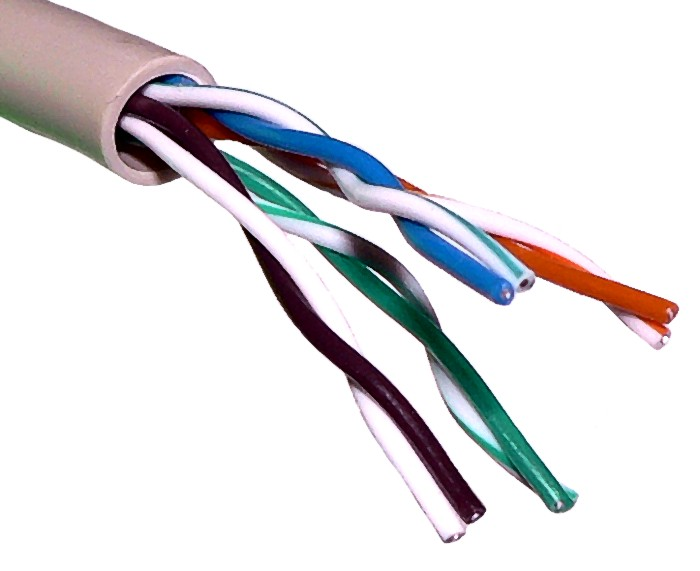
\includegraphics[width=0.6\textwidth]{images/utp_cable.jpg}%
  }{%
    \fbox{\parbox{0.85\textwidth}{Bild fehlt: \texttt{images/utp\_cable.jpg}}}%
  }%
}
\caption{Beispiel eines UTP-Kabels (Quelle: Wikimedia Commons, Datei: UTP\_cable.jpg)}
\end{figure}

\subsubsection{UTP, STP, FTP, S/FTP}
Die Bezeichnungen geben an, ob ein Gesamtschirm und/oder ein Paarschirm vorhanden ist:
\begin{itemize}
\item \textbf{U/UTP (UTP):} Kein Gesamtschirm, kein Paarschirm. Guenstig, flexibel, in Buero-/Schulumgebungen haeufig.
\item \textbf{F/UTP (oft FTP genannt):} Folien-Gesamtschirm um alle Paare.
\item \textbf{S/UTP (oft STP genannt):} Geflecht-Gesamtschirm um alle Paare.
\item \textbf{S/FTP:} Geflecht-Gesamtschirm plus Folien-Schirm je Adernpaar. Sehr gute EMV-Eigenschaften.
\end{itemize}

Abschirmung schuetzt Kabel vor Stoerquellen wie Stromleitungen, Maschinen, Funkquellen oder benachbarten Datenkabeln. Grundregel: Je staerker die Umgebung stoert (z.\,B. Industriehallen, viele leistungsstarke Geraete, lange parallele Leitungsfuehrung), desto wichtiger sind hochwertige Schirmung und saubere Erdung.

In der Praxis entscheidet die Umgebung ueber die passende Schirmungsart. In ruhigen Buero- oder Klassenraumumgebungen reicht oft UTP aus. In technischen Raeumen mit Schaltschranken, Motoren oder vielen parallel gefuehrten Leitungen ist S/FTP meist die sicherere Wahl. Wichtig ist dabei: Eine gute Schirmung wirkt nur dann optimal, wenn die gesamte Installation fachgerecht ausgefuehrt ist, also inklusive geeigneter Anschlusskomponenten und korrekter Potentialfuehrung.

\subsubsection{Cat-Standards bei Kupferkabeln}
Die Kategorie (\textit{Category}, Cat) beschreibt die Uebertragungseigenschaften der Kupferverkabelung. Sie gibt insbesondere Auskunft ueber die maximal nutzbare Frequenz, die moegliche Datenrate und damit indirekt ueber die Qualitaetsanforderungen an Kabel und Installation.

\begin{longtable}{|l|l|l|l|}
\hline
\textbf{Kategorie} & \textbf{Bandbreite} & \textbf{Typische Datenraten} & \textbf{Typische Verwendung} \\
\hline
Cat5e & 100 MHz & 1 Gbit/s bis 100 m & Standard-LAN, Schul-/Buero-Netz \\
\hline
Cat6 & 250 MHz & 1 Gbit/s bis 100 m, 10 Gbit/s bis ca. 55 m & Neuinstallationen mit Reserve \\
\hline
Cat6A & 500 MHz & 10 Gbit/s bis 100 m & Professionelle strukturierte Verkabelung \\
\hline
Cat8 & 2000 MHz & 25/40 Gbit/s bis 30 m & Rechenzentrum, kurze High-Speed-Links \\
\hline
\end{longtable}

In klassischen LAN-Installationen gilt fuer Kupferverbindungen typischerweise eine maximale Linklaenge von 100 m. In der Praxis werden heute haeufig Cat6A oder Cat7-basierte Verkabelungen eingesetzt, da sie ausreichende Reserven fuer 10-Gigabit-Anwendungen bieten.

Diese 100 m setzen sich typischerweise aus bis zu 90 m Verlegekabel und insgesamt bis zu 10 m Patchkabeln zusammen. Wird die Strecke laenger, steigt die Daempfung und die Fehlerrate kann zunehmen. Das zeigt, dass Layer 1 nicht nur von theoretischen Datenraten lebt, sondern stark von physikalischen Effekten wie Widerstand, Frequenzverhalten und Signal-Rausch-Abstand abhaengt.

\subsubsection{Farbcode T568A und T568B}
Der am weitesten verbreitete Netzwerkstecker im Kupferbereich ist RJ45 (8P8C) mit acht Pins fuer acht Adern. Fuer die Belegung sind zwei Varianten normiert: T568A und T568B. Technisch sind beide gleichwertig, entscheidend ist die \textbf{konsistente Nutzung} innerhalb einer Installation.

\begin{longtable}{|c|l|l|}
\hline
\textbf{Pin} & \textbf{T568A} & \textbf{T568B} \\
\hline
1 & Weiss/Gruen & Weiss/Orange \\
\hline
2 & Gruen & Orange \\
\hline
3 & Weiss/Orange & Weiss/Gruen \\
\hline
4 & Blau & Blau \\
\hline
5 & Weiss/Blau & Weiss/Blau \\
\hline
6 & Orange & Gruen \\
\hline
7 & Weiss/Braun & Weiss/Braun \\
\hline
8 & Braun & Braun \\
\hline
\end{longtable}

In vielen europaeischen Installationen wird T568B bevorzugt. Die Pins 1 und 2 werden klassisch als Sendeleitungen, die Pins 3 und 6 als Empfangsleitungen betrachtet (historische Sicht auf MDI-Portbelegung).

Neben RJ45 existieren im strukturierten Verkabelungsbereich auch alternative Stecksysteme wie GG45 oder TERA, die in speziellen Umgebungen eingesetzt werden. Im Alltag dominiert jedoch RJ45, weil es sehr weit verbreitet, robust und mit Ethernet-Technik ueber viele Generationen kompatibel ist. Fuer eine zuverlaessige Verbindung ist neben der richtigen Pinbelegung auch eine saubere mechanische Verarbeitung entscheidend, da schlecht gecrimpte Stecker haeufige Fehlerquellen sind.

\subsubsection{Was ist ein Crossover-Kabel?}
Ein \textit{Patchkabel} (\textit{Straight Through}) ist an beiden Enden gleich aufgelegt (A-A oder B-B). Solche Kabel werden fuer die meisten Standardverbindungen verwendet, z.\,B. PC zu Switch oder Switch zu Router.

Ein \textit{Crossover-Kabel} ist an einem Ende nach T568A und am anderen Ende nach T568B aufgelegt. Dadurch werden Sende- und Empfangsadern gekreuzt. Frueher war das fuer direkte Verbindungen gleichartiger Geraete relevant (z.\,B. PC zu PC oder Switch zu Switch). Heute erkennen viele Geraete den Leitungstyp automatisch (\textit{Auto-MDI/X}), sodass Crossover-Kabel deutlich seltener benoetigt werden.

In modernen Netzen ist es deshalb ueblich, fast ausschliesslich Patchkabel einzusetzen. Falls dennoch Verbindungsprobleme auftreten, lohnt sich ein Blick auf Layer 1: Sind die Adern korrekt aufgelegt? Ist das Kabel beschaedigt? Ist die Strecke zu lang? Viele scheinbar ``logische'' Netzwerkprobleme haben letztlich eine physikalische Ursache.

\subsection{Glasfaser (LWL)}
LWL (\textit{Lichtwellenleiter}) uebertraegt Daten als Lichtimpulse statt als elektrische Signale. Dadurch ist die Uebertragung praktisch unempfindlich gegen elektromagnetische Stoerungen und erlaubt sehr hohe Datenraten ueber grosse Distanzen. Typische Einsatzbereiche sind Backbone-Verbindungen, Verbindungen zwischen Gebaeuden, Provider-Netze und WAN-Strecken.

Eine Glasfaser besteht vereinfacht aus drei Bereichen: dem \textit{Core} (Kern), in dem das Licht gefuehrt wird, dem \textit{Cladding} (Mantel), das das Licht durch Totalreflexion im Kern haelt, und einer schuetzenden Buffer-Schicht. Eine typische Singlemode-Angabe wie 9/125 um bedeutet 9 um Kerndurchmesser und 125 um Manteldurchmesser.

Ein grosser Vorteil von LWL ist die geringe Daempfung pro Kilometer im Vergleich zu elektrischen Leitungen. Dadurch sind sehr lange Verbindungen moeglich, ohne dass in kurzen Abstaenden aktive Verstaerker noetig werden. Gleichzeitig ist Glasfaser galvanisch getrennt, was bei Potentialunterschieden zwischen Gebaeuden oder bei blitzgefuehrdeten Umgebungen ein Sicherheits- und Zuverlaessigkeitsvorteil sein kann.

\subsubsection{Singlemode vs. Multimode}
\noindent
Multimode-Fasern besitzen einen groesseren Kern (typisch 50/125 um oder 62.5/125 um). Dadurch koennen mehrere Lichtmoden gleichzeitig laufen, was die Technik guenstiger macht, aber Reichweite und maximale Datenrate staerker begrenzt. Typische Wellenlaengen liegen bei 850 nm, uebliche Einsaetze sind LAN- und Gebaeudeverkabelungen mit Strecken bis etwa einige hundert Meter.

Singlemode-Fasern besitzen einen sehr kleinen Kern (typisch 9/125 um). Es wird im Wesentlichen nur eine Lichtmode gefuehrt, wodurch deutlich hoehere Reichweiten und sehr hohe Datenraten moeglich sind. Typische Wellenlaengen sind 1310 nm und 1550 nm, eingesetzt wird Singlemode vor allem im Backbone, bei Providern und in WAN-Umgebungen.

Multimode ist besonders wirtschaftlich auf kuerzeren Strecken innerhalb von Gebaeuden oder Rechenzentren, waehrend Singlemode fuer laengere Distanzen und skalierbare Infrastruktur bevorzugt wird. Die konkrete Wahl haengt von der geplanten Strecke, den benoetigten Datenraten und den Gesamtkosten aus Transceivern, Patchfeldern und Verlegeaufwand ab. Fuer langfristige Projekte wird oft bewusst eine leistungsfaehigere Infrastruktur eingeplant, um spaetere Upgrades ohne neue Verkabelung zu ermoeglichen.

\begin{longtable}{|l|l|l|}
\hline
\textbf{Merkmal} & \textbf{Singlemode (OS1/OS2)} & \textbf{Multimode (OM1-OM5)} \\
\hline
Kerndurchmesser & ca. 9 um & 50 oder 62.5 um \\
\hline
Lichtquelle & Laser (typ. 1310/1550 nm) & LED/VCSEL (typ. 850/1300 nm) \\
\hline
Reichweite & Sehr hoch (km-Bereich) & Eher kurz bis mittel (typ. Gebaeude/DC) \\
\hline
Typischer Einsatz & Backbone, Campus, FTTH, WAN & Rechenzentrum, Inhouse-Verkabelung \\
\hline
\end{longtable}

\begin{figure}[H]
\centering
\IfFileExists{Work/Aufgaben/OSI-Modell/Layer1/images/multimode_vs_singlemode.png}{%
  
\includegraphics[width=0.75\textwidth]{Work/Aufgaben/OSI-Modell/Layer1/images/multimode_vs_singlemode.png}%
}{%
  \IfFileExists{images/multimode_vs_singlemode.png}{%
    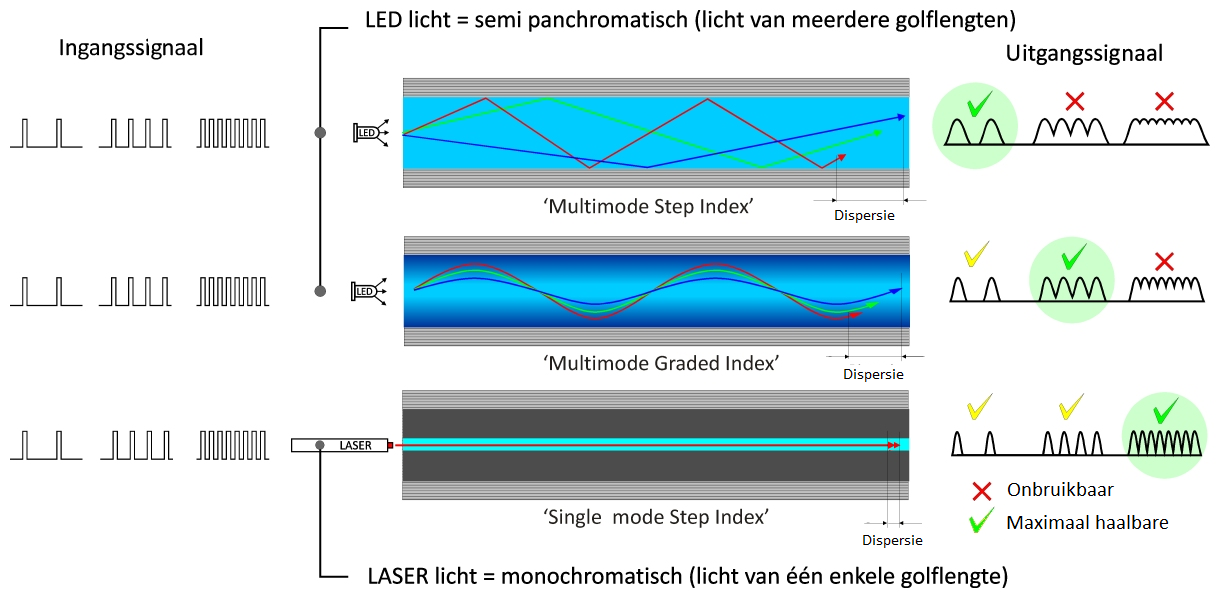
\includegraphics[width=0.75\textwidth]{images/multimode_vs_singlemode.png}%
  }{%
    \fbox{\parbox{0.85\textwidth}{Bild fehlt: \texttt{images/multimode\_vs\_singlemode.png}}}%
  }%
}
\caption{Singlemode vs. Multimode (Quelle: Wikimedia Commons, Datei: Multimode\_vs\_Single\_Mode\_Fiber.png)}
\end{figure}

\subsubsection{Vorteile und Nachteile von Glasfaser}
\begin{itemize}
\item \textbf{Vorteile:} Sehr hohe Bandbreite, grosse Reichweite, keine elektromagnetischen Stoerungen, geringe Daempfung, gute Abhoersicherheit.
\item \textbf{Nachteile:} Hoehere Kosten, empfindlichere Handhabung, aufwendigere Installation und Messtechnik.
\end{itemize}

\subsubsection{Steckertypen bei Glasfaser}
In der Praxis kommen mehrere Steckertypen vor, unter anderem LC, SC, ST, FC und E2000. Farbkennzeichnungen helfen bei der schnellen Zuordnung: Haeufig steht Blau fuer Singlemode (UPC), Gruen fuer Singlemode APC und Beige/Weiss fuer Multimode-Systeme (herstellerabhaengig).

Bei Glasfaser ist Sauberkeit ein zentrales Qualitaetskriterium. Schon kleine Verunreinigungen auf den Stirnflaechen der Stecker koennen Daempfung erhoehen oder Reflexionen verursachen. Deshalb gehoeren Sichtkontrolle, Reinigung und fachgerechte Messung (z.\,B. Daempfungsmessung) zur professionellen Inbetriebnahme und Wartung.

\subsection{Funk (WLAN)}
WLAN (\textit{Wireless Local Area Network}) nutzt auf Layer 1 elektromagnetische Wellen statt physischer Leitungen. Auch hier werden technisch betrachtet Bits uebertragen, nur eben drahtlos. WLAN basiert auf IEEE 802.11 und ermoeglicht mobile, flexible Netzzugaenge ohne Verkabelung bis zum Endgeraet.
\begin{itemize}
\item \textbf{2.4 GHz:} Gute Reichweite und Durchdringung, aber stoeranfaelliger und meist geringere nutzbare Datenrate.
\item \textbf{5 GHz:} Hoehere Datenraten, mehr Kanaele, geringere Reichweite als 2.4 GHz.
\item \textbf{6 GHz (Wi-Fi 6E/7):} Sehr viele freie Kanaele, hohe Datenraten, kurze Reichweite und hohe Daempfung.
\end{itemize}

Bei WLAN gilt grundsaetzlich: Hoehere Frequenzen bieten oft mehr Geschwindigkeit und mehr nutzbare Kanaele, haben jedoch meist eine geringere Reichweite und schlechtere Wanddurchdringung. Stoerungen entstehen unter anderem durch Waende, andere WLAN-Netze, Bluetooth-Geraete und Mikrowellen.

Im Unterschied zu Kupfer oder LWL ist Funk ein geteiltes Medium: Mehrere Geraete nutzen dieselbe Luftschnittstelle und beeinflussen sich gegenseitig. Deshalb haengt die erreichbare Datenrate nicht nur vom Standard ab, sondern stark von Kanalplanung, Abstand zum Access Point, Auslastung und Stoerquellen. Eine gute WLAN-Planung umfasst daher die Wahl geeigneter Kanaele, sinnvolle Sendeleistung, ausreichende Anzahl von Access Points und die Beruecksichtigung baulicher Gegebenheiten.

WLAN ist auf Layer 1 physikalisch einzuordnen, auch wenn in der Praxis natuerlich weitere Protokollschichten beteiligt sind. Fuer den Anwender ist besonders wichtig: Hohe Brutto-Datenraten auf dem Datenblatt bedeuten nicht automatisch dieselbe Nettoleistung im Alltag. Reale Bedingungen vor Ort sind entscheidend.

\section{Vergleich Kupfer vs. Glasfaser (LWL) vs. Funk}
\begin{longtable}{|p{2.9cm}|p{4.2cm}|p{4.2cm}|p{3.6cm}|}
\hline
\textbf{Kriterium} & \textbf{Kupfer (Twisted Pair)} & \textbf{Glasfaser (LWL)} & \textbf{Funk (WLAN)} \\
\hline
Medium & Elektrische Signale & Lichtimpulse & Funkwellen \\
\hline
Geschwindigkeit & Hoch & Sehr hoch & Mittel bis hoch (abhaengig von Standard und Umgebung) \\
\hline
Reichweite & Typisch bis 100 m & Von hunderten Metern bis viele Kilometer & Variabel, stark umgebungsabhaengig \\
\hline
Stoeranfaelligkeit & Mittel, mit Schirmung reduzierbar & Gering (EMI-unempfindlich) & Hoch, da geteiltes Medium \\
\hline
Kosten & Gering bis mittel & Hoeher & Mittel \\
\hline
\end{longtable}

Der Vergleich zeigt, dass es kein universell ``bestes'' Medium fuer alle Faelle gibt. Kupfer ist kostenguenstig, robust und fuer klassische Arbeitsplatzanschluesse sehr geeignet. Glasfaser spielt ihre Staerken bei grossen Strecken, hoher Stoersicherheit und sehr hohen Bandbreiten aus. WLAN bietet maximale Flexibilitaet und Mobilitaet, ist aber staerker von der Umgebung und der Netzplanung abhaengig.

In realen Netzwerken werden diese Medien meist kombiniert: Endgeraete nutzen WLAN oder Kupfer, Etagenverteiler sind per Kupfer oder LWL angebunden, und das zentrale Backbone wird haeufig mit Glasfaser realisiert. Diese Kombination verbindet Wirtschaftlichkeit, Leistung und Flexibilitaet.

\subsection*{Wann nimmt man was?}
\begin{itemize}
\item \textbf{Kupfer (Twisted Pair):} Arbeitsplatzverkabelung, kurze bis mittlere Strecken in Gebaeuden, gutes Preis-Leistungs-Verhaeltnis.
\item \textbf{LWL:} Backbone zwischen Verteilern/Gebaeuden, lange Strecken, hohe Bandbreite und Umgebungen mit starker EMV-Belastung.
\item \textbf{WLAN:} Mobile Endgeraete, flexible Erweiterung ohne neue Kabelwege, sinnvoll als Ergaenzung zur strukturierten Verkabelung.
\end{itemize}

\section{Zusammenfassung}
Layer 1 bildet die technische Basis jeder Netzkommunikation. Hier wird festgelegt, wie Bits physikalisch uebertragen werden, welche Medien verwendet werden und welche Grenzwerte fuer Reichweite, Stoerfestigkeit und Datenrate gelten. Obwohl diese Schicht keine Dateninhalte interpretiert, entscheidet sie wesentlich ueber die Gesamtleistung eines Netzwerks.

Aus technischer Sicht ist Layer 1 damit mehr als ``nur Kabel''. Er umfasst alle physikalischen Rahmenbedingungen, die eine Verbindung erst moeglich machen: Signalformen, Materialien, Stecksysteme, Daempfung, Abschirmung und Umgebungsbedingungen. Werden diese Punkte bei Planung und Installation sauber beruecksichtigt, arbeiten auch die hoeheren Schichten stabil und effizient.

Die Wahl des passenden Mediums entscheidet direkt ueber Reichweite, Stabilitaet, Datenrate und Kosten:
\begin{itemize}
\item Kupfer ist fuer viele Standard-LAN-Szenarien wirtschaftlich und praxisnah.
\item LWL ist bei grossen Distanzen, hohen Bandbreiten und EMV-Anforderungen klar im Vorteil.
\item WLAN erweitert Layer 1 um Mobilitaet, benoetigt aber sorgfaeltige Funkplanung.
\end{itemize}

Fuer die Praxis bedeutet das: Gute Netzwerke entstehen durch die richtige Kombination aus Medium, Topologie und sauberer Umsetzung. Gerade bei Fehlersuche, Erweiterung oder Modernisierung lohnt sich deshalb immer ein strukturierter Blick auf Layer 1.

\section*{Quellen (Auswahl)}
\begin{itemize}
\item Fluke Networks: \texttt{https://www.flukenetworks.com/knowledge-base/application-or-standards-articles-copper/differences-between-wiring-codes-t568a-vs}
\item ANSI/TIA-568 Uebersicht: \texttt{https://en.wikipedia.org/wiki/ANSI/TIA-568}
\item Eaton/Tripp Lite Ethernet Cables: \texttt{https://tripplite.eaton.com/products/ethernet-cable-types}
\item Tektronix 802.11 PHY Primer: \texttt{https://www.tek.com/en/documents/primer/wi-fi-overview-80211-physical-layer-and-transmitter-measurements}
\item Twisted Pair Grundlagen: \texttt{https://en.wikipedia.org/wiki/Twisted\_pair}
\item LWL Singlemode vs Multimode: \texttt{https://commons.wikimedia.org/wiki/File:Multimode\_vs\_Single\_Mode\_Fiber.png}
\end{itemize}

\end{document}